\documentclass[11pt,letterpaper]{article}

% ── Packages ──────────────────────────────────────────────
\usepackage[margin=1in]{geometry}
\usepackage{amsmath,amssymb}
\usepackage{mathtools}
\usepackage{booktabs}
\usepackage{enumitem}
\usepackage{hyperref}
\usepackage[dvipsnames]{xcolor}
\usepackage{titlesec}
\usepackage{microtype}
\usepackage{parskip}
\usepackage{tikz}
\usetikzlibrary{arrows.meta,positioning,calc,fit}

% ── Formatting ────────────────────────────────────────────
\hypersetup{colorlinks=true, linkcolor=NavyBlue, citecolor=NavyBlue, urlcolor=NavyBlue, pdfstartview=FitH}
\titleformat{\section}{\large\bfseries}{\thesection}{1em}{}
\titleformat{\subsection}{\normalsize\bfseries}{\thesubsection}{1em}{}
\titleformat{\subsubsection}{\normalsize\itshape}{\thesubsubsection}{1em}{}

% ── Math shortcuts ────────────────────────────────────────
\newcommand{\bfp}{\mathbf{p}}
\newcommand{\bfz}{\mathbf{z}}
\newcommand{\bfy}{\mathbf{y}}
\newcommand{\bfd}{\mathbf{d}}
\newcommand{\cS}{\mathcal{S}}
\newcommand{\R}{\mathbb{R}}
\newcommand{\pp}{\,\text{pp}}

\begin{document}

% ── Title ─────────────────────────────────────────────────
\begin{center}
{\LARGE\bfseries Neural Field Perceiver}\\[6pt]
{\large Cross-Patient Speech Decoding from Intra-Operative $\mu$ECoG\\via Reprojection-Supervised Spatial Alignment}\\[12pt]
{\normalsize Ben Tang \quad\textbar\quad Greg Cogan Lab, Duke University}\\[4pt]
{\normalsize April 2026 \quad\textbar\quad Version 9}
\end{center}

\medskip\noindent\rule{\textwidth}{0.4pt}\medskip

\noindent Technical design document for the Neural Field Perceiver.
Claims are labeled \textbf{supported by related work} (published evidence in adjacent settings, not directly validated for intra-op $\mu$ECoG), \textbf{internally observed} (our experiments), or \textbf{working hypothesis} (unverified).
Structural assumptions that could be wrong are marked in \textcolor{BrickRed}{red}.

\tableofcontents
\newpage


%% ====================================================================
%%  SECTION 1: PROBLEM
%% ====================================================================

\section{Problem}\label{sec:problem}

Each patient's $\mu$ECoG array is a sparse spatial sample of cortical activity during speech. The array sits on left ventral sensorimotor cortex (vSMC), and its position in MNI-152 space is known post-hoc from electrode reconstruction.

\textbf{Input.} For patient $i$ with $N_i$ electrodes at MNI positions $\{\bfp_j^{(i)}\}$, we observe high-gamma analytic amplitude (HGA, 70--150\,Hz) at 200\,Hz:
\begin{equation}\label{eq:observation}
d_j^{(i)}(t) = a\bigl(\bfp_j^{(i)},\; t\bigr) + \epsilon_j^{(i)}(t)
\end{equation}
where $a(\bfp, t)$ is the cortical HGA field and $\epsilon$ captures noise, impedance variation, and sub-electrode activity.

\textbf{Output.} Infer the phoneme sequence $\bfy = (y_1, y_2, y_3)$ from a 9-phoneme vocabulary --- three separate 9-way classifications per non-word token (e.g., /a/, /b/, /e/).

\textbf{Cross-patient challenge.} Electrode $j$ on patient $i$ and electrode $j$ on patient $i'$ sample different cortical locations. Arrays are offset 15--25\,mm in MNI with variable rotation. Channel indices are meaningless across patients.

\begin{table}[ht!]
\centering\small
\begin{tabular}{@{}llr@{}}
\toprule
\textbf{Constraint} & \textbf{Value} & \textbf{Impact} \\
\midrule
Electrodes/patient & 63--201 & Sparse cortical sampling \\
Electrode spacing & ${\sim}2$\,mm & Near-columnar resolution \\
Cross-patient offset & 15--25\,mm & Different regions sampled \\
Trials/patient & 46--178 & Small-data regime \\
Utterance/patient & ${\sim}1$\,min & Too little for SSL \\
Phonemes & 9 classes $\times$ 3 positions & Low-dimensional output \\
\bottomrule
\end{tabular}
\end{table}


%% ====================================================================
%%  SECTION 2: KEY IDEA
%% ====================================================================

\section{Key Idea: Shared Neural Field + Reprojection}\label{sec:idea}

\subsection{Decomposition}

Cross-patient decoding requires shared structure. We decompose each patient's cortical field:
\begin{equation}\label{eq:decomposition}
a^{(i)}(\bfp, t) = f\bigl(T_i(\bfp),\; t;\; \bfy\bigr) + r^{(i)}(\bfp, t)
\end{equation}
\begin{itemize}[leftmargin=2em]
\item $f$: shared neural field --- the spatiotemporal pattern phoneme $\bfy$ produces in canonical cortical space.
\item $T_i$: patient-specific spatial transform (estimated by MNI normalization, imperfect).
\item $r^{(i)}$: patient-specific residual (individual neural organization, signal quality, pathology).
\end{itemize}
Cross-patient decoding works to the extent that $\|f\| \gg \|r^{(i)}\|$.

\subsection{The factorization}\label{sec:factorization}

The shared field $f$ factorizes through a low-dimensional bottleneck:
\begin{equation}\label{eq:obs-function}
d_j^{(i)}(t) = g\bigl(\bfp_j^{(i)},\; \bfz(t)\bigr) + r^{(i)}\bigl(\bfp_j^{(i)},\; t\bigr) + \epsilon_j^{(i)}(t)
\end{equation}
where:
\begin{itemize}[leftmargin=2em]
\item $g(\bfp, \bfz)$: the \textbf{somatotopic map} --- given a brain position and an articulatory state, what is the neural activity? Time-invariant: lip motor cortex encodes lip state the same way at $t{=}0$ and $t{=}500$\,ms. Absorbs all spatial dependence.
\item $\bfz(t) \in \R^k$ ($k {\approx} 5$--$8$): the \textbf{articulatory state} --- tongue position, lip aperture, voicing, etc. Absorbs all time and phoneme dependence.
\item $\dot{\bfz}(t) = h(\bfz(t); \bfy)$: dynamics on the articulatory manifold.
\end{itemize}
Space and time interact only through the $k$-dimensional bottleneck $\bfz(t)$. Instead of learning every (position $\times$ time $\times$ phoneme) combination, the model learns a spatial basis $g$ and temporal dynamics $h$ composed through $\bfz$. This is what makes the problem tractable with 63--201 electrodes.

\textbf{The somatotopic map is static.} $g$ does not change during a trial. Cross-patient alignment is therefore a static geometric problem: different patients have electrodes at different positions sampling the same map. The temporal dynamics $\bfz(t)$ are shared across patients --- the same phoneme produces similar trajectories regardless of who speaks it.

\subsection{The 3D vision analogy}\label{sec:analogy}

This structure maps to multi-view 3D reconstruction:

\begin{table}[ht!]\centering\small
\begin{tabular}{@{}ll@{}}
\toprule
\textbf{3D Reconstruction} & \textbf{Neural Field Decoding} \\
\midrule
3D body model & Shared somatotopic map $g(\bfp, \bfz)$ \\
Pose parameters & Articulatory state $\bfz(t)$ \\
Camera extrinsics & MNI offset $\Delta^{(i)}$, rotation $\omega^{(i)}$ \\
Camera intrinsics & Per-patient gain/bias \\
2D keypoints & Electrode observations $d_j^{(i)}(t)$ \\
\textbf{Reprojection loss} $\|\pi(V) - x\|^2$ & \textbf{Reprojection loss} $\|g(\bfp, \hat{\bfz}) - d\|^2$ \\
\bottomrule
\end{tabular}
\end{table}

\textbf{Reprojection loss}: if your latent state estimate is correct, you should predict what every electrode observes. Self-supervised but geometrically grounded --- unlike JEPA/VICReg/masked reconstruction, the target is physically meaningful.

\textbf{Where the analogy breaks.} (1) Each patient is a different ``scene,'' not a different camera on the same scene --- the shared structure is weaker than photometric consistency. (2) We have 63--201 electrodes, not 65K pixels --- the reprojection signal per frame is thin. (3) The ``scene'' changes every frame. These mean reprojection is a useful regularizer, not the primary signal. The supervised classification loss remains primary.

\subsection{Evidence and central hypothesis}

\textbf{Central hypothesis.} \textit{Intra-operative $\mu$ECoG speech recordings share enough spatiotemporal structure across patients that a coordinate-aware spatial encoder, trained with reprojection supervision, will improve cross-patient phoneme decoding beyond methods that treat each patient's electrode array as unrelated.} This is testable via ablation A1 (Section~\ref{sec:ablations}). The document designs an architecture to test this hypothesis; it does not assume the hypothesis is true.

\textbf{Supported by related work.}
Per-patient input layers + shared backbone transfers in adjacent settings: Singh~\cite{singh2025} ($N{=}25$ sEEG, PER 0.49 group vs.\ 0.57 individual); Willett~\cite{willett2023} (per-day affine + shared GRU).
Articulatory somatotopy in vSMC is reproducible~\cite{metzger2023,bouchard2013}.
Motor manifold structure is preserved across individuals~\cite{safaie2023,gallego2020}.
MNI coordinates improve cross-patient ECoG transfer: Chen~\cite{chen2025} (SwinTW, PCC 0.765 on unseen patients).%
\footnote{Standard ECoG (10\,mm spacing), not $\mu$ECoG (2\,mm). None of these results use intra-operative recordings, $\mu$ECoG resolution, or our small-data regime. They support the general direction, not the specific formulation.}

\textbf{Internally observed.}
LOPO achieves PER\,=\,0.762 on S14 (frozen backbone, grouped-by-token CV) --- above chance (0.89) but worse than per-patient (0.737).
55 experiments converge to PER 0.750--0.780, suggesting a systematic barrier (data scarcity, alignment, or both --- not yet isolated).
Articulatory bottleneck head improves LOPO decoding, consistent with $f$ organized along articulatory dimensions.


%% ====================================================================
%%  SECTION 3: ARCHITECTURE
%% ====================================================================

\section{Architecture}\label{sec:architecture}

The model prediction is:
\begin{equation}\label{eq:implemented}
\boxed{\hat{d}_j^{(i)}(t) = g_\theta\bigl(\tilde{\bfp}_j^{(i)},\; s^{(i)}(t),\; e^{(i)}\bigr)}
\end{equation}
where $\tilde{\bfp}_j^{(i)}$ is the corrected electrode position, $s^{(i)}(t) \in \R^{L \times d}$ is the spatial representation ($L{=}16$ virtual electrodes), and $e^{(i)}$ is a patient embedding. This is deterministic; the observation model $d = \hat{d} + \epsilon$ separates prediction from noise.

\textcolor{BrickRed}{\textit{Theory--implementation gap:}} Unlike the idealized Eq.~\ref{eq:obs-function}, the implemented model conditions on patient identity through $e^{(i)}$. This is a deliberate relaxation to handle the patient-specific residual $r^{(i)}$, but it creates an escape hatch: the decoder can use $e^{(i)}$ to explain observations without the latent state $s$ becoming patient-invariant. To mitigate this, $\mathcal{L}_{\text{cross}}$ zeroes out the patient embedding (Section~\ref{sec:obs-decoder}), forcing cross-patient reconstruction to succeed without patient identity. The within-patient $\mathcal{L}_{\text{reproj}}$ retains $e^{(i)}$. The three losses create a gradient tension: $\mathcal{L}_{\text{reproj}}$ rewards patient-specific structure; $\mathcal{L}_{\text{cross}}$ rewards patient-invariant structure; $\mathcal{L}_{\text{class}}$ rewards whatever predicts phonemes. Ablation A5 tests whether this tension helps or hurts.

\subsection{Overview}

\begin{center}
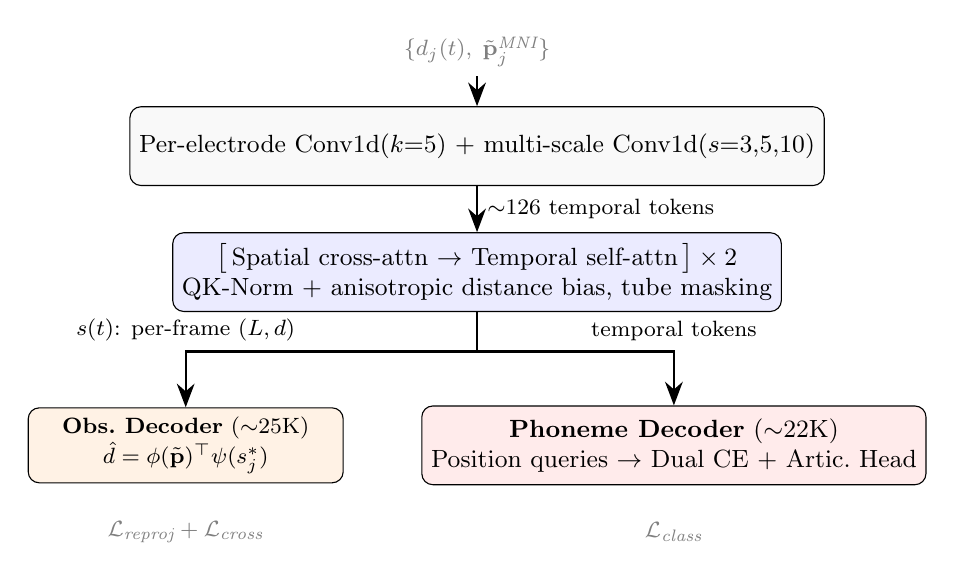
\begin{tikzpicture}[
  box/.style={draw, rounded corners, minimum width=5.5cm, minimum height=1cm, align=center, font=\small},
  smallbox/.style={draw, rounded corners, minimum width=4cm, minimum height=0.8cm, align=center, font=\footnotesize},
  arrow/.style={-{Stealth[length=3mm]}, thick},
  label/.style={font=\footnotesize\itshape, text=gray}
]

\node[box, fill=gray!5] (input) at (0, 0.8) {Per-electrode Conv1d($k{=}5$) + multi-scale Conv1d($s{=}3{,}5{,}10$)};

\node[box, fill=blue!8] (block) at (0, -0.8) {$\bigl[$\,Spatial cross-attn $\to$ Temporal self-attn\,$\bigr] \times 2$\\QK-Norm + anisotropic distance bias, tube masking};

\node[smallbox, fill=orange!10] (obs) at (-3.7, -3.0) {\textbf{Obs.\ Decoder} (${\sim}$25K)\\$\hat{d} = \phi(\tilde{\bfp})^\top\psi(s_j^*)$};

\node[box, fill=red!8] (phoneme) at (2.5, -3.0) {\textbf{Phoneme Decoder} (${\sim}$22K)\\Position queries $\to$ Dual CE + Artic.\ Head};

\node[label] (raw) at (0, 2.0) {$\{d_j(t),\; \tilde{\bfp}_j^{\text{MNI}}\}$};

\draw[arrow] (raw) -- (input);
\draw[arrow] (input) -- (block) node[midway, right, font=\footnotesize] {${\sim}126$ temporal tokens};
\draw[arrow] (block.south) -- ++(0,-0.5) -| (obs.north) node[midway, above, font=\footnotesize] {$s(t)$: per-frame $(L,d)$};
\draw[arrow] (block.south) -- ++(0,-0.5) -| (phoneme.north) node[midway, above, font=\footnotesize] {temporal tokens};

\node[label] at (-3.7, -4.1) {$\mathcal{L}_{\text{reproj}} + \mathcal{L}_{\text{cross}}$};
\node[label] at (2.5, -4.1) {$\mathcal{L}_{\text{class}}$};

\end{tikzpicture}
\end{center}

\begin{equation}
\boxed{\mathcal{L} = \mathcal{L}_{\text{class}} + \lambda_1 \mathcal{L}_{\text{reproj}} + \lambda_2 \mathcal{L}_{\text{cross}}, \qquad \lambda_1{:}\; 0.5 {\to} 0.1,\quad \lambda_2{:}\; 0.3 {\to} 0.05}
\end{equation}

\textbf{Factorized interleaved processing} replaces strict spatial$\to$temporal separation. Each layer alternates spatial cross-attention (virtual electrodes aggregate from real electrodes within a time window) and temporal self-attention (each virtual electrode attends across time windows). The spatial distance bias is \textbf{static} --- the same at every time step --- respecting the time-invariance of $g$ (Section~\ref{sec:factorization}). Temporal attention captures dynamics in $\bfz(t)$. Interleaving lets temporal context denoise spatial estimates at every layer.

Two representations:
\begin{itemize}[leftmargin=2em]
\item $s(t) \in \R^{L \times d}$: virtual electrode outputs after spatial cross-attention. Used by the observation decoder for reprojection.
\item $\bfz_p \in \R^d$: per-phoneme-position readout via learned query cross-attention over temporal tokens. Used for classification.
\end{itemize}


\subsection{Electrode Tokens}\label{sec:tokens}

For electrode $j$ on patient $i$ at time $t$:
\begin{equation}
\text{token}_j = \underbrace{\text{Linear}(d_j \to d)}_{\text{activity}} + \underbrace{\text{Linear}\bigl(\gamma(\tilde{\bfp}_j) \to d\bigr)}_{\text{Fourier MNI PE}} + \underbrace{e^{(i)}}_{\text{patient}}
\end{equation}
where $\tilde{\bfp}_j = R(\omega^{(i)}) \cdot \bfp_j + \Delta^{(i)}$ is the corrected MNI position.

\textbf{Fourier positional encoding.} Following NeRF~\cite{mildenhall2020}, \textbf{standardized} MNI coordinates (zero-mean, scaled so the speech motor region spans $[{-}1, 1]$ per axis) pass through multi-scale sinusoidal features before projection:
\begin{equation}
\gamma(\bar{\bfp}) = \bigl[\sin(2^0 \pi \bar{\bfp}),\; \cos(2^0 \pi \bar{\bfp}),\; \ldots,\; \sin(2^{F-1} \pi \bar{\bfp}),\; \cos(2^{F-1} \pi \bar{\bfp})\bigr] \in \R^{6F}
\end{equation}
with $F{=}4$ frequency levels. MNI coordinates are standardized \textbf{before} encoding: the speech motor region spans ${\sim}30$\,mm per axis, so $\bar{\bfp} \in [{-}1, 1]$ maps 1 unit $\approx 15$\,mm. The resulting wavelengths are $\lambda_\ell = 2/2^\ell$ in standardized units: $\ell{=}0 \to 30$\,mm (full-array), $\ell{=}1 \to 15$\,mm (articulatory region), $\ell{=}2 \to 7.5$\,mm (sub-region), $\ell{=}3 \to 3.75$\,mm (near electrode spacing). A linear projection $\text{Linear}(24 \to d)$ maps to token dimension.%
\footnote{NeRF uses $F{=}10$ for sub-pixel detail. We use $F{=}4$ because (a) ${\sim}200$ electrode positions across ${\sim}20$ patients cannot constrain higher frequencies, and (b) the finest wavelength ($3.75$\,mm) already approaches electrode spacing (${\sim}2$\,mm). Finer frequencies risk encoding noise rather than structure.}

\textbf{Per-patient parameters} ($6 + d$ per patient):
\begin{itemize}[leftmargin=2em]
\item $\Delta^{(i)} \in \R^3$: translation (init $\mathbf{0}$). Corrects placement offset.
\item $\omega^{(i)} \in \R^3$: axis-angle rotation (init $\mathbf{0}$, Rodrigues formula). Corrects orientation.
\item $e^{(i)} \in \R^d$: patient embedding (init $\sim \mathcal{N}(0, 0.02)$). Absorbs residual $r^{(i)}$.
\end{itemize}

\textcolor{BrickRed}{\textit{Assumption:} $e^{(i)}$ is added uniformly to all tokens --- the encoder cannot make position-dependent patient corrections. Only the decoder can (via $\text{MLP}(\tilde{\bfp}, e)$). For tumors with spatially non-uniform distortion, this is a known limitation.}


\subsection{Temporal Preprocessing}

\textbf{Per-electrode denoising.} Conv1d($k{=}5$, stride${=}1$) on each electrode's time series provides ${\sim}25$\,ms temporal smoothing.

\textbf{Multi-scale tokenization.} Three parallel Conv1d branches at strides 3, 5, 10 (sampling intervals 15, 25, 50\,ms) on each denoised electrode time series. The branches provide three temporal resolutions; what temporal structure each one captures depends on the kernel size, downstream attention, and data --- not on the stride alone. Tokenization uses the production window $[0, T_{\text{utt}}]$ (${\approx}1.0$\,s, 200 samples at 200\,Hz): stride 3 yields 66 tokens, stride 5 yields 40, stride 10 yields 20, totaling ${\approx}126$ temporal tokens per electrode. Concatenated with learnable per-scale embeddings + sinusoidal temporal PE (encoding each token's center time in seconds).


\subsection{Virtual Electrodes}\label{sec:virtual-electrodes}

$L = 16$ learned query vectors at learned MNI positions. Fixed model parameters, the same for every patient and time step. During spatial cross-attention, each virtual electrode attends to all real electrodes, weighted by spatial proximity.

After cross-attention, virtual electrode $\ell$ holds a $d$-dimensional summary of cortical activity near its position. The output $s(t) \in \R^{L \times d}$ is a spatially-indexed representation in a shared frame --- every patient maps to the same 16 positions regardless of electrode count or grid layout.

\textbf{Atlas initialization.} Virtual electrode positions are initialized at Brainnetome atlas~\cite{fan2016} centroids of speech motor subregions: lip M1, tongue M1, jaw M1, laryngeal M1, lip S1, tongue S1, ventral premotor, supplementary motor area, and adjacent somatosensory zones. This gives anatomically meaningful starting positions so backprop only needs to fine-tune, not discover cortical organization from scratch. Repulsive regularization $\mathcal{L}_{\text{repel}} = \sum_{i \neq j} \max(0, r_{\min} - \|\text{v\_pos}_i - \text{v\_pos}_j\|)$ prevents collapse.

\textbf{Why 16.} 63--201 electrodes cover ${\sim}20 \times 30$\,mm. 16 virtual electrodes gives ${\sim}5$\,mm spacing, roughly matching somatotopic scale. Ablation A4 tests $\{4, 8, 16, 32\}$.

\textbf{Coverage gaps.} Virtual electrodes in uncovered cortical regions receive only weak, distant attention and will drift toward covered regions or produce noise. The union of all patients' coverage is larger than any single patient's --- more patients and cross-task pooling expand the coverage envelope. No architecture fixes missing data.


\subsection{Interleaved Spatiotemporal Blocks ($\times 2$)}\label{sec:interleaved}

Each block alternates two attention operations:

\textbf{(a) Spatial cross-attention} (per temporal window). Virtual electrodes (Q) attend to real electrode tokens (K, V) within each time window. Attention logits use \textbf{QK-Norm} + \textbf{anisotropic distance bias}:
\begin{equation}
A_{ij} = \tau_h \cdot \frac{Q_i \cdot K_j}{\|Q_i\|\,\|K_j\|} \;-\; (\bar{\bfp}_i - \bar{\bfp}_j)^\top \Sigma_i^{-1} (\bar{\bfp}_i - \bar{\bfp}_j)
\end{equation}
where $\tau_h > 0$ is a learnable temperature per head (init $\sqrt{d_h}$, clamped $\leq 100$), $\bar{\bfp}$ denotes standardized MNI coordinates, and $\Sigma_i = C_i C_i^\top$ is a per-virtual-electrode covariance ($C_i$: lower-triangular Cholesky factor, 6 params each, init $\alpha I$). Normalizing Q and K to unit vectors keeps the content term bounded, so the distance bias has a consistent effect throughout training regardless of embedding norms --- following SwinV2~\cite{chen2025} and ViT-22B. Each virtual electrode learns the \textbf{shape} of its spatial receptive field: an elongated lip region, a compact tongue area, etc. 96 + 4 params ($16 \times 6$ covariances $+$ 4 temperatures). 4-head attention.

The distance bias is \textbf{static}: $\Sigma_i$ depends only on virtual electrode identity, not on time or input content. The spatial geometry of attention is the same at every time step, consistent with $g$ being time-invariant. What changes with time are the \textbf{values} (electrode activity), not the spatial weighting structure.

\textbf{(b) Temporal self-attention} (per virtual electrode). Each of the 16 virtual electrodes attends across all ${\sim}126$ temporal tokens. 4 heads, sinusoidal temporal PE + per-scale embeddings. This captures articulatory dynamics $h(\bfz; \bfy)$.

Optional 1-layer spatial self-attention between virtual electrodes within each time window (captures inter-zone co-articulation, e.g., simultaneous lip rounding and tongue backing).

\textbf{Block internals.} Each sub-layer uses Pre-LayerNorm: $\text{out} = x + \text{SubLayer}(\text{LN}(x))$. The FFN after each attention operation is SwiGLU~\cite{shazeer2020}:
\begin{equation}
\text{FFN}(x) = \bigl(x W_1 \odot \text{SiLU}(x W_{\text{gate}})\bigr) W_2, \qquad W_1, W_{\text{gate}} \in \R^{d \times d_{\text{ff}}},\; W_2 \in \R^{d_{\text{ff}} \times d}
\end{equation}
with $d_{\text{ff}} = \lfloor 8d/3 \rfloor$, matching the parameter count of a standard $4d$ ReLU FFN. Dropout $p{=}0.2$ on attention weights and FFN output. DropPath $p{=}0.1$ on the residual stream. Each block thus contains: LN $\to$ spatial cross-attn $\to$ LN $\to$ FFN $\to$ LN $\to$ temporal self-attn $\to$ LN $\to$ FFN.

\textbf{Tube masking.} Instead of masking electrodes independently per frame, mask each selected electrode across a contiguous time window of 5--10 frames ($25$--$50$\,ms). Masking is \textbf{scale-consistent}: when electrode $j$ is masked at time $t$, it is masked at all three temporal resolutions simultaneously. Otherwise the model trivially reconstructs masked information from a finer or coarser scale --- the somatotopic map $g(\bfp, \bfz)$ is the same physical function at every temporal resolution. This forces interpolation in \textbf{both} space (from nearby electrodes at the same time) \textbf{and} time (from the same electrode at adjacent windows), exercising both types of shared structure.

\textbf{Masking curriculum.} Start at 30\%, anneal to 70\% over training. Low masking early helps the spatial encoder learn basic distance-activity relationships. High masking later forces robust spatial interpolation. The somatotopic map is spatially smooth (${\sim}5$\,mm scale), so 70\% masking is physically feasible.

\textbf{Spatial readout.} Attention pooling (not MaxPool) preserves the somatotopic decomposition:
\begin{equation}
s_{\text{pool}}(t) = \sum_{i=1}^{L} w_i \cdot \text{out}_i(t), \qquad w_i = \text{softmax}\bigl(\mathbf{q}_{\text{read}}^\top \text{out}_i(t) / \sqrt{d}\bigr)
\end{equation}

\textbf{Per-position readout via learned queries.} Three learned query vectors $\mathbf{q}_p \in \R^d$ ($p \in \{1,2,3\}$) cross-attend to the full spatially-pooled temporal token sequence:
\begin{equation}
\bfz_p = \text{CrossAttn}\bigl(\mathbf{q}_p,\; K{=}\{s_{\text{pool}}(t)\}_{t},\; V{=}\{s_{\text{pool}}(t)\}_{t}\bigr)
\end{equation}
Each query discovers where its phoneme's information concentrates in the temporal sequence, accounting for variable phoneme durations, coarticulation across boundaries, and CVC/VCV structural asymmetry (VCV: 0.68\,s vs.\ CVC: 0.58\,s~\cite{duraivel2025}). Inspired by DETR's object queries~\cite{carion2020}, which learn to attend to task-relevant regions without hard spatial partitioning. Ablation A13 compares against fixed equal-window averaging. Global readout $z_{\text{global}} = \text{mean}(\text{all temporal tokens})$ for $k$-NN.


\subsection{Why Perceiver, not ViT or point-cloud methods?}

\textbf{ViT} requires a fixed regular grid. Our patients have different grid sizes (8$\times$16, 12$\times$22) at different MNI positions. Cannot use.

\textbf{Point-cloud methods} (PointNet~\cite{qi2017}, Point Transformer~\cite{zhao2021}) handle irregular 3D point sets and are legitimate alternatives. Perceiver cross-attention is simpler for our case: shared query vectors directly provide the fixed-size shared output we need, and our 63--201 points are too small for hierarchical architectures. Worth testing as an ablation.


\subsection{Observation Decoder (${\sim}$25K params)}\label{sec:obs-decoder}

The forward model --- predicts what each electrode should observe given the latent state. Structurally, this is a DeepONet~\cite{lu2021}: a branch network encodes the latent field, a trunk network encodes spatial position, and they interact through a low-rank inner product. The neural operator literature validates this as the right inductive bias for sparse field reconstruction.

\textbf{Position-weighted aggregation.} Each electrode $j$ gets a local latent by weighting virtual electrode outputs by spatial proximity:
\begin{equation}
s_j^*(t) = \sum_{\ell=1}^{L} a_{j\ell} \cdot \text{out}_\ell(t), \qquad
a_{j\ell} = \frac{\exp\bigl(-\alpha_{\text{dec}} \cdot \|\bar{\tilde{\bfp}}_j - \bar{\text{v\_pos}}_\ell\|^2\bigr)}
             {\sum_{m} \exp\bigl(-\alpha_{\text{dec}} \cdot \|\bar{\tilde{\bfp}}_j - \bar{\text{v\_pos}}_m\|^2\bigr)}
\end{equation}

\textbf{Bilinear prediction.}
\begin{equation}\label{eq:bilinear}
\hat{d}_j^{(i)}(t) = \phi(\tilde{\bfp}_j,\; e^{(i)})^\top \;\psi\bigl(s_j^*(t)\bigr)
\end{equation}
$\phi = \text{MLP}_{\text{spatial}}(\tilde{\bfp}, e) \in \R^k$: spatial tuning (trunk). $\psi = \text{MLP}_{\text{latent}}(s_j^*) \in \R^k$: latent activation (branch). $k{=}32$.

Unlike the encoder (where $e^{(i)}$ is a global bias), the decoder's $\phi(\tilde{\bfp}, e)$ learns position-dependent patient effects --- partially modeling the nonlinear residual $\delta_i(\bfp)$. Ablation A9 tests a full MLP fallback.

\textbf{Within-patient reprojection loss.}
\begin{equation}
\mathcal{L}_{\text{reproj}} = \frac{1}{N_i T} \sum_{t,j} \bigl\| d_j(t) - \hat{d}_j(t) \bigr\|^2
\end{equation}
Computed over all electrodes including masked ones (the model must interpolate).

\textbf{Cross-patient reprojection loss.}\label{sec:cross-reproj}
During multi-patient training, when patients $A$ and $B$ have trials with the same phoneme sequence, the shared observation function should explain \textbf{both} patients' observations from either patient's latent state. For each matched pair, both observations and latents are averaged over the matching phoneme window:
\begin{equation}
\mathcal{L}_{\text{cross}} = \frac{1}{N_B} \sum_{j=1}^{N_B} \bigl\| \bar{d}_j^{(B)} - g_\theta(\tilde{\bfp}_j^{(B)},\; \bar{s}_A^{*,(B)},\; \mathbf{0}) \bigr\|^2
\end{equation}
where $\bar{d}_j^{(B)} = \tfrac{1}{|W|}\sum_{t \in W} d_j^{(B)}(t)$ is patient $B$'s observation averaged over the phoneme window $W$, and $\bar{s}_A^{*,(B)} = \tfrac{1}{|W|}\sum_{t \in W} s_A^{*,(B)}(t)$ aggregates patient $A$'s window-averaged virtual electrode outputs at patient $B$'s electrode positions. \textbf{The patient embedding is set to $\mathbf{0}$} --- the decoder must predict patient $B$'s observations using only spatial position and patient $A$'s latent, with no patient-identity shortcut.

This design prevents the escape hatch where the decoder uses $e^{(B)}$ to explain cross-patient variance without the latent becoming patient-invariant. The three losses create a deliberate tension:
\begin{itemize}[leftmargin=2em]
\item $\mathcal{L}_{\text{reproj}}$: with $e^{(i)}$ --- rewards patient-specific reconstruction.
\item $\mathcal{L}_{\text{cross}}$: with $e{=}\mathbf{0}$ --- rewards patient-invariant spatial structure.
\item $\mathcal{L}_{\text{class}}$: rewards whatever predicts phonemes.
\end{itemize}

\textcolor{BrickRed}{\textit{Caution:} Cross-patient reprojection is noisier than within-patient because (1)~the patient residuals $r^{(A)} \neq r^{(B)}$ mean a perfect $g$ still leaves unexplained variance, and (2)~window-averaging blurs temporal dynamics within the phoneme. Weight $\lambda_2 < \lambda_1$ and anneal aggressively. If $\mathcal{L}_{\text{cross}}$ competes with $\mathcal{L}_{\text{class}}$, the $\lambda_2{=}0$ fallback drops it entirely.}

\textbf{Optional: Beta-NLL.} Replace MSE with learned per-electrode variance to downweight noisy electrodes:
\begin{equation}
\mathcal{L}_{\text{reproj}}^{\text{UQ}} = \frac{1}{2}\Bigl(\log \hat{\sigma}_j^2 + \frac{(d_j - \hat{d}_j)^2}{\hat{\sigma}_j^2}\Bigr) \cdot \bigl(\hat{\sigma}_j^2\bigr)^{0.5}_{\text{sg}}
\end{equation}


\subsection{Phoneme Decoder (${\sim}$5K params)}

Dual head per position $p \in \{1,2,3\}$:
\begin{equation}
\text{logits}_p = \frac{1}{2}\bigl(\underbrace{\text{Linear}(z_p \to 9)}_{\text{CE head}} + \underbrace{\tau \cdot \text{normalize}(\text{Linear}(z_p \to 15)) \cdot A^\top}_{\text{articulatory head}}\bigr)
\end{equation}
$A \in \R^{9 \times 15}$: fixed articulatory feature matrix. $\tau$: learnable temperature. Separate heads per position.

$\mathcal{L}_{\text{class}} = \frac{1}{3}\sum_{p} \text{FocalCE}(\text{logits}_p, y_p;\; \gamma{=}2, \text{LS}{=}0.1)$ with mixup ($\alpha{=}0.2$).


\subsection{Parameter Budget}

\begin{table}[ht!]\centering\small
\begin{tabular}{@{}lrll@{}}
\toprule
\textbf{Module} & \textbf{Params} & \textbf{Shared?} & \textbf{Role} \\
\midrule
Interleaved blocks ($\times 2$) & ${\sim}$160K & Shared & Spatial inversion + dynamics \\
\quad incl.\ anisotropic $\Sigma_i$ + $\tau_h$ & 100 & Shared & Receptive field shape + QK temp \\
\quad incl.\ virtual positions & 48 & Shared & Atlas-initialized MNI coords \\
Position queries + cross-attn & ${\sim}$17K & Shared & Learned phoneme readout \\
Observation decoder & ${\sim}$25K & Shared & Reprojection forward model \\
Phoneme dual heads ($\times 3$) & ${\sim}$5K & Shared & Classification \\
Multi-scale Conv1d & ${\sim}$12K & Shared & Temporal tokenization \\
\midrule
$\Delta^{(i)} + \omega^{(i)} + e^{(i)}$ & 70/pt & Per-patient & Registration + identity \\
\midrule
\textbf{Total shared} & $\mathbf{{\sim}219}$\textbf{K} & & \\
\textbf{Grand total} (10 pts) & $\mathbf{{\sim}220}$\textbf{K} & & (cf.\ current: 122K) \\
\bottomrule
\end{tabular}
\end{table}


%% ====================================================================
%%  SECTION 4: TRAINING AND EVALUATION
%% ====================================================================

\section{Training and Evaluation}\label{sec:training}

\subsection{Phase 1: Source training}

$N{-}1$ source patients (where $N$ is the total PS cohort; exact count depends on LOPO target). Each batch:
\begin{enumerate}[leftmargin=2em]
\item Construct tokens with Fourier MNI PE. Apply tube masking (curriculum 30$\to$70\%).
\item Interleaved blocks: spatial cross-attn $\to$ temporal self-attn $\times 2$.
\item Within-patient reprojection on all electrodes (including masked) $\to \mathcal{L}_{\text{reproj}}$.
\item Cross-patient reprojection on same-token trial pairs $\to \mathcal{L}_{\text{cross}}$.
\item Per-position readout $\to$ dual head $\to \mathcal{L}_{\text{class}}$.
\item $\mathcal{L} = \mathcal{L}_{\text{class}} + \lambda_1 \mathcal{L}_{\text{reproj}} + \lambda_2 \mathcal{L}_{\text{cross}}$.
\end{enumerate}

AdamW with differential LR: shared params $10^{-3}$; geometric params ($\Delta, \omega$, virtual positions, $\Sigma$) $3 {\times} 10^{-4}$; patient $e$ at $10^{-3}$. Linear warmup (20 epochs) $\to$ cosine decay. Weight decay $10^{-4}$, grad clip 5.0, batch 16. Early stopping on held-out 20\% source validation, patience 7.

\subsection{Phase 2: Target adaptation (LP-FT)}

Per fold of 5-fold grouped-by-token CV on target patient:
\begin{enumerate}[leftmargin=2em]
\item \textbf{Linear probe.} Freeze encoder, train decoder + $\Delta^{(\text{target})} + \omega^{(\text{target})} + e^{(\text{target})}$. 150 epochs. Best checkpoint by inner validation (20\% held out from training fold).
\item \textbf{Fine-tune.} Unfreeze encoder at $0.1\times$ LR. 100 epochs, patience 7.
\end{enumerate}

\subsection{Phase 3 (optional): Transductive reprojection pre-training}

Pre-train spatial encoder + decoder using $\mathcal{L}_{\text{reproj}}$ only. If target patient's unlabeled data is included, this is transductive and must be reported separately from strict LOPO.

\subsection{Evaluation regimes}

\begin{enumerate}[leftmargin=2em]
\item \textbf{Zero-shot.} Phase 1 only. $\Delta = \mathbf{0}$, $\omega = \mathbf{0}$, $e = \text{mean}(e^{(\text{source})})$, all frozen. Strongest claim, likely worst PER.
\item \textbf{LP-FT (primary).} Phase 1 $\to$ Phase 2. Matches clinical calibration scenario.
\item \textbf{Transductive.} Phase 3 $\to$ Phase 1 $\to$ Phase 2. Reported separately.
\end{enumerate}

\textbf{Metrics.} PER (edit distance), grouped-by-token 5-fold CV. Full recipe: weighted $k$-NN ($k{=}10$, cosine), TTA 16, dual head, source $k$-NN at $0.5\times$ weight. Conformal prediction sets as interpretability output.


%% ====================================================================
%%  SECTION 5: WHAT OUR EXPERIMENTS SHOW
%% ====================================================================

\section{What Our Experiments Show}\label{sec:experiments}

\subsection{Evaluation recipe matters more than architecture}

\begin{table}[ht!]
\centering\small
\begin{tabular}{@{}llrr@{}}
\toprule
\textbf{Component added} & \textbf{Category} & \textbf{PER} & \textbf{$\Delta$} \\
\midrule
Baseline (CE, mean-pool) & -- & 0.872 & -- \\
+ Label smoothing 0.1 & Training & 0.831 & $-4.1\pp$ \\
+ Per-position heads + dropout & Training & 0.819 & $-1.2\pp$ \\
+ Mixup $\alpha{=}0.2$ & Training & 0.802 & $-1.7\pp$ \\
+ Weighted $k$-NN ($k{=}10$) & Evaluation & 0.781 & $-2.1\pp$ \\
+ TTA (16 copies) & Evaluation & 0.767 & $-1.4\pp$ \\
+ Articulatory + CE dual head & Model & 0.737 & $-3.0\pp$ \\
\bottomrule
\end{tabular}
\end{table}

Cumulative, not independent. Total: $-13.5\pp$. All on S14, grouped-by-token CV. Per-fold noise is $\pm 0.05$ PER, so improvements $< 2\pp$ may not replicate.

\subsection{Multi-scale temporal: largest observed architectural gain}

Stride 3+5+10 gave PER $0.766 \to 0.750$ ($-1.6\pp$), the largest single-change gain from any architectural modification. However, this is below the $\pm 5\pp$ per-fold noise floor and needs multi-seed replication to confirm. Validated on BiGRU; needs re-validation on transformer.

\subsection{The ${\sim}0.76$ convergence}

55 LOPO experiments converge to PER 0.750--0.780. Not attributable to any single bottleneck: S14 is no longer truly held out (55+ architectures evaluated); ${\sim}30$ samples/fold give $\pm 0.05$ noise; S14 has only 153 trials; spatial alignment is one factor among several.

\subsection{SSL failed at this data scale}

All SSL methods near chance (PER 0.85--0.91). JEPA + LP-FT: 0.797. With ${\sim}1$\,min utterance/patient, SSL cannot learn useful representations from HGA.


%% ====================================================================
%%  SECTION 6: ABLATION PLAN
%% ====================================================================

\section{Ablation Plan}\label{sec:ablations}

\begin{table}[ht!]\centering\small
\begin{tabular}{@{}clp{6.8cm}@{}}
\toprule
\textbf{ID} & \textbf{Ablation} & \textbf{Question} \\
\midrule
A1 & MNI PE present/absent & \textbf{Central}: do coordinates help? \\
 & \quad a. Current Conv2d+BiGRU baseline & $\to$ 0.762 (LP-FT) \\
 & \quad b. Perceiver, random positions & $\to$ architecture benefit \\
 & \quad c. Perceiver + Fourier MNI PE & $\to$ MNI benefit \\
 & \quad d. (c) + reprojection loss & $\to$ reprojection benefit \\
 & \quad e. (d) + cross-patient reproj.\ & $\to$ cross-patient benefit \\
\midrule
A2 & Population-level (all patients) & Is the 0.76 wall S14-specific? \\
A3 & Per-patient params & $\Delta$ only / $+\omega$ / $+e$ / pos-dep $e$ \\
A4 & Virtual electrode count & $L \in \{4, 8, 16, 32\}$ \\
A5 & Reprojection weight & $\lambda_1, \lambda_2 \in \{0, 0.01, 0.1, 0.5\}$ \\
A6 & Cross-task pooling & $+$ Duraivel 2025 data \\
A7 & Reprojection loss variant & Beta-NLL vs.\ MSE \\
A8 & Spatial attention & Isotropic $\alpha$ vs.\ anisotropic $\Sigma_i$ \\
A9 & Bilinear vs.\ MLP decoder & $\phi^\top\psi$ vs.\ MLP$([\tilde{\bfp}; e; s_j^*])$ \\
A10 & Interleaved vs.\ separated & Interleaved blocks vs.\ strict spatial$\to$temporal \\
A11 & Masking strategy & Tube vs.\ per-frame; masking ratio 30--80\% \\
A12 & Fourier PE vs.\ linear PE & $\gamma(\bfp)$ vs.\ $\text{Linear}(\bfp \to d)$ \\
A13 & Position readout & Learned queries vs.\ fixed equal-window averaging \\
\bottomrule
\end{tabular}
\end{table}


%% ====================================================================
%%  SECTION 7: PRIORITIES AND RISKS
%% ====================================================================

\section{Priorities and Risks}\label{sec:priorities}

\subsection{Priority ordering}

The document's own evidence suggests:

\begin{enumerate}[leftmargin=2em]
\item \textbf{Cross-task data pooling (A6).} Lowest risk. Same phonemes, overlapping patients~\cite{duraivel2025}. Directly addresses data scarcity. Works with current pipeline and new architecture.

\item \textbf{Population-level evaluation (A2).} Pure methodology fix. Required to distinguish S14-specific effects from universal trends. Must be the primary success criterion.

\item \textbf{MNI coordinate architecture (A1, this document).} Highest novelty, highest risk. The hypothesis that spatial alignment is the binding constraint is plausible but unvalidated --- it has not been isolated from data scarcity or measurement noise.
\end{enumerate}

\subsection{Success criteria}

\textbf{Primary:} Mean PER across all patients improves over current LOPO baseline ($\geq 3$ seeds, LP-FT regime). MNI benefit isolated by paired comparisons: A1c vs.\ A1b (MNI value) and A1d vs.\ A1c (reprojection value).

\textbf{Interpretability (weak evidence):} Virtual electrode positions cluster over known speech motor regions --- but since positions are atlas-initialized, this partly reflects initialization bias, not learned structure. Stronger evidence: positions that \textit{move away} from atlas priors in a somatotopically coherent direction. Spatial tuning vectors $\phi(\bfp)$ recover articulatory somatotopy. Learned $\Delta^{(i)}$ and $\omega^{(i)}$ correlate with known registration quality.

\subsection{Risks}

\begin{table}[ht!]\centering\small
\begin{tabular}{@{}p{0.35\textwidth}cp{0.42\textwidth}@{}}
\toprule
\textbf{Risk} & \textbf{Severity} & \textbf{Mitigation} \\
\midrule
MNI coordinates unavailable & High & Fallback to scaled grid positions (ablation A1b tests random-init) \\
MNI alignment too imprecise & High & Ablation A1; learnable $\alpha$ adapts \\
Reprojection competes with classification & Med & $\lambda$ ablation A5; $\lambda{=}0$ fallback \\
Perceiver overfits (200K, 1300 trials) & Med & Masking; early stopping; reproj.\ reg. \\
Bilinear separability too restrictive & Med & Ablation A9: MLP fallback \\
Rigid $(\Delta,\omega)$ too crude for surgical brains & Med & $e^{(i)}$ absorbs non-geometric residuals; if insufficient, test pos-dep $e$ (A3) \\
Virtual electrodes collapse & Low & Atlas init; repulsive regularization \\
\bottomrule
\end{tabular}
\end{table}


%% ====================================================================
%%  SECTION 8: DATA
%% ====================================================================

\section{Available Data}\label{sec:data}

\begin{table}[ht!]\centering\small
\begin{tabular}{@{}lllcc@{}}
\toprule
\textbf{Cohort} & \textbf{Patients} & \textbf{Trials} & \textbf{MNI?} & \textbf{Usage} \\
\midrule
PS (Spalding published) & 8 patients$^\dagger$ & ${\sim}$1096 & Expected$^*$ & Source / target \\
PS (additional) & S16, S57$^\dagger$ & ${\sim}$250 & Expected$^*$ & Source \\
Cross-task (Duraivel 2025) & 3 overlapping pts & 156--208/pt & Expected$^*$ & Priority 1 \\
Lexical task & 13 patients & Varies & Expected$^*$ & Future source \\
\midrule
\textbf{Total unique PS} & \textbf{10 patients} & $\mathbf{{\sim}1350}$ & & \\
\bottomrule
\end{tabular}
\end{table}

\noindent $^\dagger$S32 = S36 (duplicate, counted once). 12 PS entries in BIDS $\to$ 11 unique $\to$ 10 usable (S18 excluded). The 8 Spalding patients include S14 (153 trials), used as Phase 2 target in pilot results. For LOPO, source = $N{-}1$ patients.

\noindent $^*$MNI coordinates available from BioImage Suite (DBS) / Brainlab (tumor) outputs on Box.%
\footnote{\textbf{Hard gate:} All MNI-dependent claims (Fourier PE, $\Delta/\omega$ correction, cross-patient reprojection) are conditional on extracting and auditing these coordinates. Fallback: scaled grid positions (retains within-patient structure, loses cross-patient alignment). Ablation A1 tests with and without coordinates.}


% ── Bibliography ──────────────────────────────────────────
\begin{thebibliography}{99}\raggedright

\bibitem{singh2025}
Singh, A., et al.\ (2025).
Transfer learning via distributed brain recordings enables reliable speech decoding.
\textit{Nature Communications}, 16, 8749.

\bibitem{willett2023}
Willett, F.R., et al.\ (2023).
A high-performance speech neuroprosthesis.
\textit{Nature}, 620, 1031--1036.

\bibitem{metzger2023}
Metzger, S.L., et al.\ (2023).
A high-performance neuroprosthesis for speech decoding and avatar control.
\textit{Nature}, 620, 1037--1046.

\bibitem{bouchard2013}
Bouchard, K.E., et al.\ (2013).
Functional organization of human sensorimotor cortex for speech articulation.
\textit{Nature}, 495, 327--332.

\bibitem{safaie2023}
Safaie, M., et al.\ (2023).
Preserved neural dynamics across animals performing similar behaviour.
\textit{Nature Neuroscience}, 26, 714--724.

\bibitem{gallego2020}
Gallego, J.A., et al.\ (2020).
Long-term stability of cortical population dynamics underlying consistent behavior.
\textit{Nature Neuroscience}, 23, 260--270.

\bibitem{chen2025}
Chen, J., et al.\ (2025).
Transformer-based neural speech decoding from surface and depth electrode signals.
\textit{Journal of Neural Engineering}, 22(1), 016017.

\bibitem{wu2025}
Wu, R., et al.\ (2025).
Across-speaker articulatory reconstruction from sensorimotor cortex.
\textit{bioRxiv}. doi:10.1101/2025.10.08.680888

\bibitem{spalding2025}
Spalding, Z., et al.\ (2025).
Shared latent representations of speech production for cross-patient speech decoding.
\textit{bioRxiv}. doi:10.1101/2025.08.21.671516

\bibitem{duraivel2025}
Duraivel, S., et al.\ (2025).
Distinct neural processes link speech planning and execution.
\textit{bioRxiv}. doi:10.1101/2024.10.07.617122

\bibitem{wang2025}
Wang, J., et al.\ (2025).
VGGT: Visual Geometry Grounded Transformer.
\textit{CVPR 2025}. arXiv:2503.11651

\bibitem{xiong2024}
Xiong, Z., et al.\ (2024).
MMGN: Multi-scale multi-modal graph network for spatiotemporal field reconstruction.
\textit{ICLR 2024}.

\bibitem{truong2023}
Truong, P., et al.\ (2023).
SPARF: Neural radiance fields from sparse and noisy poses.
\textit{CVPR 2023}.

\bibitem{santos2023}
Santos, J.E., et al.\ (2023).
Development of the Senseiver for efficient field reconstruction from sparse observations.
\textit{Nature Machine Intelligence}, 5, 1317--1325.

\bibitem{qi2017}
Qi, C.R., et al.\ (2017).
PointNet: Deep learning on point sets for 3D classification and segmentation.
\textit{CVPR 2017}.

\bibitem{zhao2021}
Zhao, H., et al.\ (2021).
Point Transformer.
\textit{ICCV 2021}.

\bibitem{mildenhall2020}
Mildenhall, B., et al.\ (2020).
NeRF: Representing scenes as neural radiance fields for view synthesis.
\textit{ECCV 2020}. (Fourier positional encoding.)

\bibitem{lu2021}
Lu, L., Jin, P., Pang, G., Zhang, Z., \& Karniadakis, G.E.\ (2021).
Learning nonlinear operators via DeepONet.
\textit{Nature Machine Intelligence}, 3, 218--229.

\bibitem{fan2016}
Fan, L., et al.\ (2016).
The Human Brainnetome Atlas: A new brain atlas based on connectional architecture.
\textit{Cerebral Cortex}, 26(8), 3508--3526.

\bibitem{seitzer2022}
Seitzer, M., et al.\ (2022).
On the pitfalls of heteroscedastic uncertainty estimation with probabilistic neural networks.
\textit{ICLR 2022}.

\bibitem{angelopoulos2021}
Angelopoulos, A.N.\ \& Bates, S.\ (2021).
A gentle introduction to conformal prediction.
\textit{arXiv:2107.07511}.

\bibitem{gal2016}
Gal, Y.\ \& Ghahramani, Z.\ (2016).
Dropout as a Bayesian approximation.
\textit{ICML 2016}.

\bibitem{carion2020}
Carion, N., et al.\ (2020).
End-to-end object detection with Transformers (DETR).
\textit{ECCV 2020}.

\bibitem{shazeer2020}
Shazeer, N.\ (2020).
GLU variants improve Transformer.
\textit{arXiv:2002.05202}.

\end{thebibliography}

\end{document}
